\begin{marginfigure} % MARGIN FIGURE
\begin{center}
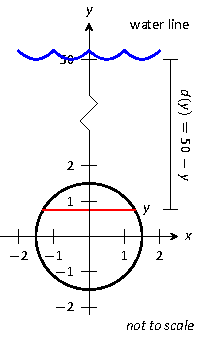
\includegraphics{figures/figfluid4}
\end{center}
\caption{Measuring the fluid force on an underwater porthole in Example \ref{eg:6.5.9}.} \label{F:6.5.porthole}
\end{marginfigure}

\begin{example} \label{eg:6.5.9} % EXAMPLE
An underwater observation tower is being built with circular viewing portholes enabling visitors to see underwater life. Each vertically oriented porthole is to have a 3 ft diameter whose center is to be located 50 ft underwater. Find the total fluid force exerted on each porthole. Also, compute the fluid force on a horizontally oriented porthole that is under 50 ft of water.

\solution
We place the center of the porthole at the origin, meaning the surface of the water is at $y=50$ and the depth function will be $d(y)=50-y$; see Figure \ref{F:6.5.porthole} 

The equation of a circle with a radius of 1.5 is $x^2+y^2=2.25$; solving for $x$ we have $x=\pm \sqrt{2.25-y^2}$, where the positive square root corresponds to the right side of the circle and the negative square root corresponds to the left side of the circle. Thus the length function at depth $y$ is $\ell(y) = 2\sqrt{2.25-y^2}$. Integrating on $[-1.5,1.5]$ we have:
\begin{align*}
F 		&= 62.4\int_{-1.5}^{1.5} 2(50-y)\sqrt{2.25-y^2}\ dy \\
			&= 62.4\int_{-1.5}^{1.5} \big(100\sqrt{2.25-y^2} - 2y\sqrt{2.25-y^2}\big)\ dy \\
			&= 6240\int_{-1.5}^{1.5} \big(\sqrt{2.25-y^2}\big)\ dy - 62.4\int_{-1.5}^{1.5} \big(2y\sqrt{2.25-y^2}\big)\ dy \\
\end{align*}			
The second integral above can be evaluated using Substitution. Let $u=2.25-y^2$ with $du = -2y\,dy$. The new bounds are: $u(-1.5)=0$ and $u(1.5)=0$; the new integral will integrate from $u=0$ to $u=0$, hence the integral is 0.

The first integral above finds the area of half a circle of radius 1.5, thus the first integral evaluates to $6240\cdot\pi\cdot1.5^2/2 = 22,054$. Thus the total fluid force on a vertically oriented porthole is $22,054$ lb.

Finding the force on a horizontally oriented porthole is more straightforward:
$$F = \text{Pressure}\times\text{Area} = 62.4\cdot50\times \pi\cdot1.5^2 = 22,054\text{ lb}.$$
That these two forces are equal is not coincidental; it turns out that the fluid force applied to a vertically oriented circle whose center is at depth $d$ is the same as force applied to a horizontally oriented circle at depth $d$.
\end{example}